\documentclass[conference,a4paper]{IEEEtran}
\usepackage[UTF8,fontset=fandol,scheme=plain]{ctex}
\usepackage{newtxtext,newtxmath}
\usepackage{graphicx,booktabs,amsmath,url}
\usepackage[hidelinks]{hyperref}
\graphicspath{{figures/}}
% Auto-generated from verified data.
\newcommand{\GateMinUs}{124.116}
\newcommand{\GateMaxUs}{484.548}
\newcommand{\HostGateKiB}{6.00}
\newcommand{\HostSoftMinKiB}{21.62}
\newcommand{\HostSoftMaxKiB}{164.25}
\newcommand{\HostReductionMin}{72.3}
\newcommand{\HostReductionMax}{96.3}
\newcommand{\QueryMinUs}{14.456}
\newcommand{\QueryMaxUs}{14.720}
\newcommand{\AreaMM}{0.321366}
\newcommand{\BankAreaPct}{84.6}
\newcommand{\SetupSlackPs}{0.313}
\newcommand{\HoldSlackPs}{-51.082}
\newcommand{\LeafCells}{222656}
\newcommand{\RtlCases}{24}
\newcommand{\RtlQueries}{72}

\hyphenation{VORTEX HardFloat StorageStacked}
\title{Logic Die 上的 MoBA 驻留门控：\\架构设计与在线验证\\
\large Resident MoBA Gating on a Memory Logic Die: Architecture and Online Validation}
\author{\IEEEauthorblockN{匿名技术稿}
\IEEEauthorblockA{可复现研究原型 \quad 2026 年 9 月}}
\begin{document}
\maketitle

\begin{abstract}
Block-sparse attention requires a gating stage that summarizes keys, scores blocks, and selects a causal subset.
This paper implements that stage on the logic die of a stacked-memory system.
A descriptor engine prepares resident BF16 key means, reuses them across queries, and returns deterministic Top-K results.
Epoch-qualified residency and a blocking completion window connect the accelerator to a real VORTEX instruction stream through AXI and a behavioral UCIe link.
The same synthesizable RTL is used in unit tests and the online SystemC model.
For 32 blocks, 128 dimensions, Top-12, and four queries, measured host request span remains
\HostGateKiB{} KiB across block sizes 1--16, compared with \HostSoftMinKiB{}--\HostSoftMaxKiB{} KiB for a scalar VORTEX reference.
End-to-end offload intervals are \GateMinUs{}--\GateMaxUs{} microseconds.
Standard-cell synthesis, numerical corner cases, and independent transaction checks expose both implementation cost and remaining timing limitations.
The results establish a memory-side gating prototype, without assuming a characterized SRAM compute macro or claiming full-model inference speedup.
\end{abstract}

\begin{IEEEkeywords}
Logic Die，MoBA，堆叠存储，BF16，驻留计算，在线联合仿真
\end{IEEEkeywords}

\section{引言}
长上下文注意力的计算量与数据搬运量推动了块稀疏算法的发展。MoBA
以键向量的块均值表示一个历史块，通过查询与块均值的相似度选择参与注意力计算的块\cite{moba}。
这种方法减少了后续注意力覆盖的块数，但增加了均值池化、打分与 Top-K 门控步骤。
门控需要访问存储中的 K，而输出只包含少量块索引。因此，门控电路的放置位置会影响
K 数据是否需要穿过处理器与存储之间的接口。

王瑞泰的学位论文提出面向 MoBA 的异构芯粒存算设计，采用 K 阶段特征提取、
Q 阶段驻留查询与基数筛选，并讨论了共享存储及 GQA 复用\cite{wang2026}。
本文以其算法分解为设计来源，把门控闭环放置在堆叠存储的 Logic Die 上，
并将放置方式落实到可执行的主机接口、本地 DMA、RTL 时序与错误处理。
图~\ref{fig:concept} 展示其位置关系。本文研究对象是门控算子；返回索引后的
注意力矩阵计算、Softmax、V 聚合与完整模型推理不在实现范围内。

本文完成三项工作：
\begin{enumerate}
\item 设计存储侧 PREPARE/QUERY 接口，使 K 的池化与 Kmean 驻留发生在 Logic Die 内，
并用 epoch 和形状匹配限定多查询复用的有效条件。
\item 实现四 bank BF16 权重数据流、FP32 顺序累加、因果掩码和稳定基数 Top-K；
完成窗口允许主机等待结果，同时保留本地 DMA 的前进路径。
\item 建立真实 VORTEX 指令执行、AXI/UCIe 在线传输、同一份门控 RTL 和原生存储时序的闭环，
提供独立数值对拍、事务记分板、负向控制及标准单元综合证据。
\end{enumerate}
这些贡献属于 Logic Die 上的架构与系统实现。BF16 计算、均值池化和 Top-K 算法本身
均有既有来源，本文不将其重新命名为新算法，也不把数字权重存储等同于物理 SRAM 存算宏。

\begin{figure}[t]
\centering
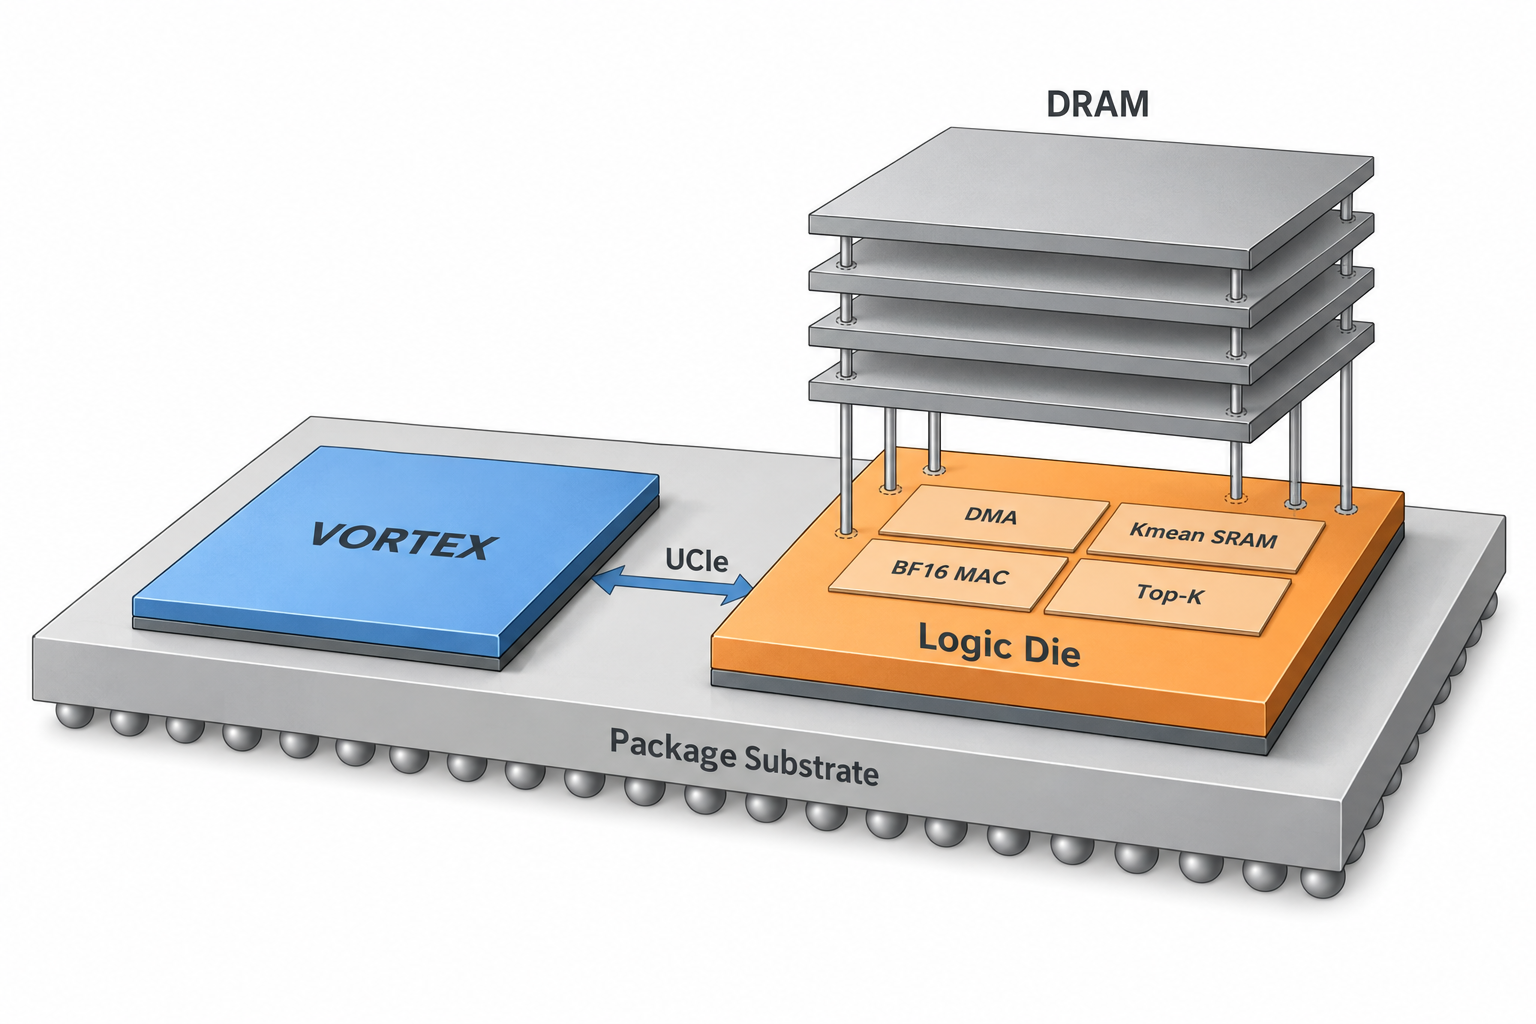
\includegraphics[width=\columnwidth]{logic_die_concept.png}
\caption{存储堆叠与 Logic Die 门控的概念位置图。使用内置图像生成工具辅助绘制；
图中几何形状不表示芯片版图、面积比例或制造结果。完整提示词随代码提供。}
\label{fig:concept}
\end{figure}

\section{背景、来源与问题定义}
\subsection{MoBA 门控及其数值契约}
设共有 $C$ 个块，每块 $B$ 个 token，头维度为 $D$。输入键为
$K_{c,t,d}$，查询为 $q_d$，当前查询所在块号为 $c_0$。门控的数学形式为
\begin{align}
\bar K_{c,d} &= \frac{1}{B}\sum_{t=0}^{B-1}K_{c,t,d},\\
s_c &= \sum_{d=0}^{D-1}q_d\bar K_{c,d}, \quad c<c_0,\\
\mathcal S &= \{c_0\}\cup\operatorname{TopK}_{k'}\{s_c:c<c_0\},\label{eq:causal}\\
k'&=\min(k-1,c_0).
\end{align}
式~\eqref{eq:causal} 使当前块必选、未来块不可选。当前块内部的 token 级因果掩码
仍须由后续注意力内核处理。$k$ 表示包含当前块的总选择上限。

为了使硬件和软件可逐结果比较，本文另行规定有限精度运算顺序。K 与 Q 为 BF16；
池化从 FP32 正零开始，按 token 顺序逐项相加；乘以 $2^{-\log_2 B}$ 后以
round-to-nearest, ties-to-even（RNE）转换为 BF16。点积按维度顺序累加，
乘法和加法分别舍入到 FP32，不融合为 FMA。BF16 子正规数不刷新为零。
非有限输入或非有限累加结果使命令失败。这是原型的数值契约，尚未评估其相对于
完整 MoBA 模型的量化误差及选择集合变化。

\subsection{与参考设计及相关工作的关系}
参考学位论文把大规模 SRAM 计算 Cell 组织为 Group/Cluster/Cell，
并以文献宏为黑盒估计存算单元指标\cite{wang2026}。
本文没有该宏的电路、版图与表征数据，因此采用可综合数字存储接口，并把权重存储
映射为标准单元寄存器。本文没有移植参考设计的三层片上网络，也不沿用其归一化工艺、
吞吐率或能效数值。

NeuPIMs 等工作研究了 NPU 与 PIM 协同执行不同类型的 LLM 运算\cite{neupims}，
说明异构计算与存储侧数据复用已有充分研究背景。本文关注更窄的问题：
在已有堆叠存储行为模型中，使 MoBA 门控拥有完整的描述符语义、可复用状态与可核验的在线接口。
VORTEX 提供开放的 RISC-V GPGPU 实现\cite{vortex}；本文使用其真实 Processor
执行程序，但实验内核仅启用一个 lane，软件时间只作为当前配置的标量参考。

\section{Logic Die 架构}
\subsection{系统边界与在线数据路径}
图~\ref{fig:architecture} 给出实际模块关系。系统基于 StorageStacked\cite{storage}，
由 VORTEX SimX、AXI256 主机、AXI2Flit、UCIe 行为链路、存储侧目标端口、
Logic Die 包装器和在线 mem\_sim 组成。VORTEX 的末级缓存后端将真实 MemReq
提交到外部接口；请求被拒绝时留在原队列头，读数据仅在链路响应返回后释放。
系统没有以离线地址回放或预生成流量代替处理器执行。

主机队列最多保存 16 条请求，VORTEX 外部在途表有 32 项。当前 AXI 主机将一条
64 B 请求串行拆为两个 256 bit beat，使用 10 bit ID 并允许回卷复用。
存储侧最多保留 4 个主机 burst，本地 DMA 最多保留一条 32 B 请求；
两类请求在原生存储 tick 上进行轮询仲裁。该实现以可观测的有界队列建立功能和时序基线，
尚未通过增加在途数量对带宽进行优化。

全部组件由单个 SystemC 内核调度，时间分辨率为 1 fs。VORTEX/AXI 周期为 2 ns，
门控 RTL 周期为 4 ns，存储按 250000 fs 的原生 tick 推进。
跨模块延迟通过实际排队、链路传送和存储完成决定；包装器不能提前返回本地副本。

\begin{figure*}[t]
\centering
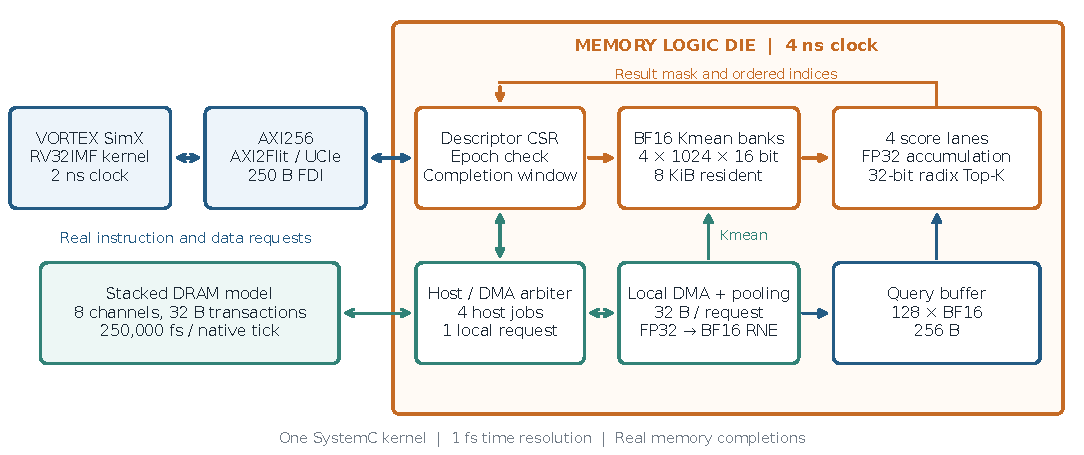
\includegraphics[width=\textwidth]{architecture.pdf}
\caption{实际在线系统与 Logic Die 模块关系，由 Python 绘制。主机访问和本地 DMA 共享存储仲裁；
Kmean 通过本地池化写入权重 bank。图中权重 bank 的默认综合实现为寄存器阵列。}
\label{fig:architecture}
\end{figure*}

\subsection{描述符与驻留生命周期}
PREPARE 描述符包含 K 基址、块数、块大小的 $\log_2$ 和 epoch。
引擎按 $[c][t][d]$ 的连续布局读取 K，逐块清零 128 个 FP32 累加槽，
完成池化后把均值写入权重 bank。默认 $C=32,D=128$，总权重容量为
$32\times128\times16$ bit，即 8 KiB。四个 bank 各为 $1024\times16$ bit，
块 $c$ 落在 bank $c\bmod4$ 中。附加池化、Q 和分数缓冲分别为 512 B、256 B 和 128 B。

驻留状态的签名为
\begin{equation}
\Sigma=(\mathrm{epoch},\mathrm{Kbase},C,\log_2 B).
\end{equation}
只有 PREPARE 全部成功后才发布 resident。QUERY 要求当前签名与成功驻留签名一致，
随后只读取 256 B 的 Q。任何 PREPARE 启动或 DMA 故障都会撤销 resident；
参数失配的 QUERY 在发起数据访问前返回错误。软件修改 K 后必须增加 epoch 并重新 PREPARE。
本接口不提供缓存侦听一致性，因此调用方须保证 K/Q 已对存储可见。

这种生命周期支持同一 KV 头供多个 Q 头复用。若 $H$ 个查询共享 K，
一次准备后的本地输入数据量为
\begin{equation}
V_{\rm local}=2CBD+2HD\quad\text{bytes}.\label{eq:traffic}
\end{equation}
该式只计有效 K/Q 输入，不包含主机描述符、指令、完成状态与结果回传。
实验的软件参考同样只池化一次并复用均值，以免将重复池化误计为硬件收益。

\subsection{四 bank 打分与稳定基数筛选}
QUERY 将 128 维 Q 保存到本地缓冲。引擎每组同时处理四个历史块，
每一维使用同步读、乘法、累加三个周期，再以一个周期写回该组分数。
不计 Q 读取及筛选阶段，打分周期为
\begin{equation}
N_{\rm score}=\left\lceil\frac{c_0}{4}\right\rceil(3D+1).
\end{equation}
因此 $c_0=31,D=128$ 时需要 3080 个周期。标准 FP32 运算复用
Berkeley HardFloat\cite{hardfloat}；控制器、数据布局、同步权重接口和基数选择控制在本项目实现。

Top-K 对有限 FP32 数执行保序变换。先将正负零统一为正零，再将非负数最高位翻转、
负数全部位取反。对变换后的无符号键从高位到低位竞争：若当前候选中存在该位为 1 的键，
仅保留这些候选，否则全部保留。扫描 32 bit 后选择最小块号作为胜者，再从可选集合中移除。
该规则使正负零同分、同分时较小块号优先，且不依赖综合器对比较树的组织。

每个胜者需要 32 个扫描时钟，整个筛选还包含启动和交接周期。
本文明确采用这一逐位时序；参考论文中“逐 bit 扫描”与“每周期一个胜者”的不同表述
没有被合并为未经实现的吞吐率假设。

\subsection{完成窗口与错误语义}
门控寄存器位于 VORTEX 不可缓存 I/O 区间内的 \texttt{0xf000--0xf3ff}。
软件写入命令后，可读取 \texttt{0xf300} 完成窗口。若引擎 busy，包装器保留该读请求；
引擎完成后返回状态，随后可读取掩码、个数和计数器。等待占用主机响应槽，
本地 DMA 则继续通过独立请求路径参与仲裁，从而使完成事件能解除等待。
当前实现没有轮询循环，也没有以软件 sleep 估计设备完成时间。

普通状态寄存器始终可读。busy 期间写寄存器、部分字节写、非法命令和尺寸均返回
SLVERR 且不修改配置。命令执行中的数据错误终止命令并置位 error。
结果索引 0 为当前块，后续索引按历史块分数降序排列。
系统复位需要共同复位和排空链路；本工作仅验证冷复位，不支持运行中任意模块单独热复位。

\section{实现与验证方法}
\subsection{可复现配置}
表~\ref{tab:config} 汇总运行条件。源代码锁定上游版本，必要的 VORTEX 修改以补丁保存。
门控单元测试与系统仿真链接同一份 Verilator 生成模型，DC 读取同一 RTL。
实验快照记录运行源文件、工作负载二进制、依赖版本和参考 PDF 的 SHA-256；
论文数据收集脚本在导出图表前再次验证源文件与综合输入哈希。

\begin{table}[t]
\caption{原型与实验条件}
\label{tab:config}\centering\small
\begin{tabular}{@{}ll@{}}
\toprule
项目 & 本文配置\\\midrule
VORTEX & RV32IMF；单活跃 lane；2 ns\\
Logic Die & $C\le32,D=128$；四 bank；4 ns\\
数据类型 & BF16 输入及权重；FP32 运算，RNE\\
主实验 & $C=32,k=12,H=4,B=1,2,4,8,16$\\
测试数据 & 正态分布确定性种子；双模式共用输入\\
外部接口 & 64 B 请求；AXI256；250 B FDI\\
存储模型 & HBM4 行为预设；8 通道；32 B 事务\\
存储时间 & tick=250000 fs；tCK=500 ps\\
映射窗口 & 64 MiB；底层模型容量 8 GiB\\
DC 条件 & 28 nm HPC+；TT，0.9 V，25\,$^\circ$C\\
时序约束 & 4 ns；不确定度 0.1 ns；I/O 延迟 0.2 ns\\
\bottomrule
\end{tabular}
\end{table}

HBM4 预设有 23 项 provisional 时序。该模型适合在公开配置下研究排队与数据路径，
但不是特定量产 HBM 的性能保证。UCIe 同样为行为模型，未完成协议或 PHY 认证。
主实验缩小了块内 token 数以控制含波形的在线仿真成本；四个块、$B=4096$ 的边界另在 RTL 层验证。
主实验不代表 $32\times4096$ token 的完整应用运行。

\begin{figure*}[t]
\centering
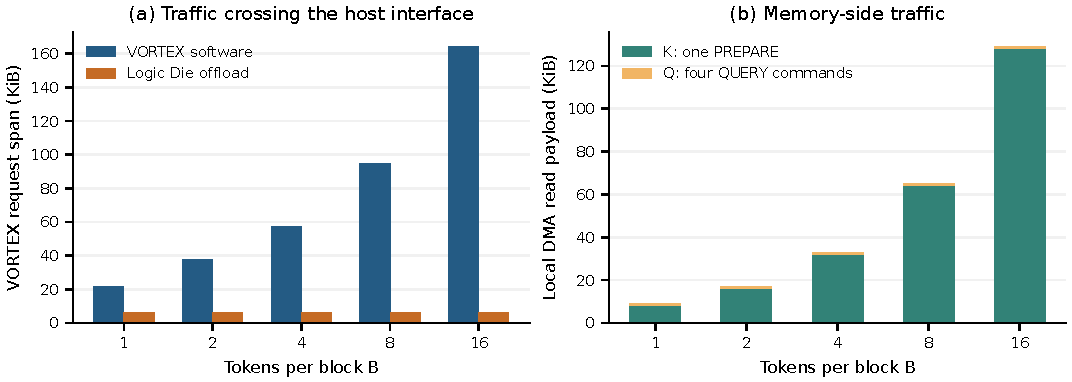
\includegraphics[width=\textwidth]{traffic.pdf}
\caption{32 块、128 维、Top-12、四次查询的实测流量。左：处理器末级请求跨度，
包括带字节使能的完整 64 B 请求；右：Logic Die 有效 DMA 读数据。
两者分别衡量外部接口占用和本地输入读取，不宜直接相加为物理链路字节数。}
\label{fig:traffic}
\end{figure*}

\subsection{独立数值与故障验证}
NumPy 参考独立执行规定的 FP32 顺序运算和 BF16 RNE，然后以数值排序得到期望集合。
RTL 测试核对掩码、个数与索引顺序，并随机改变 DMA ready 和响应延迟，
检查背压期间请求地址稳定、无重复接收及不提前完成。
\RtlCases{} 个用例包含 \RtlQueries{} 次正常查询，覆盖随机值、同分、负分、
最早因果位置、$k$ 边界、不满四块的末组、子正规数、舍入边界和 4096-token 块。
测试还检查驻留复用、epoch 失配、非法寄存器写、非有限输入、打分溢出和 DMA 故障恢复。
这些用例均通过；它们是定向与随机测试，不能替代形式化穷举证明。

系统每次用同一 AXI 路径加载程序及输入，并将这部分事务标记为 loader。
内核开始后分别运行 Logic Die 卸载和 VORTEX 软件模式。软件采用相同运算顺序，
编译禁用 FMA 融合与 fast-math。实际执行结束后，验收邮箱核对内核返回的掩码与个数。
该邮箱只用于测试参数和观察，不承担门控运算。

\subsection{跨层事务证据}
在线 PASS 之外，离线检查器执行以下独立检查：
\begin{enumerate}
\item 对两端 FDI 的实际字节逐项配对，用独立 CRC-16 实现验证 256 B 物理帧及其
250 B 有效载荷的散布位置；
\item 从 AXI 握手日志重建内存内容，核对主机读取与本地 DMA 数据；
\item 配对原生存储提交及完成事件，检查响应不早于存储完成时刻；
\item 对 VCD 中 AXI 五通道的有效握手计数，与 CSV 记录逐通道比较。
\end{enumerate}
验收还执行 8 个原生存储测试、在线 C ABI 队列/掩码/边界测试，以及多位宽
AXI/UCIe 全链路和重放回归。负向控制分别损坏参考掩码与接收 Flit 字节，
两者均被检查器捕获并返回失败。缺少在线、离线或 DRAM/DFI 结果时，不导出该用例为论文数据。

\section{实验结果与分析}
\subsection{处理器侧流量与本地读取}
图~\ref{fig:traffic} 比较两种执行模式。处理器侧统计从内核启动到全部响应排空之间
VORTEX 末级请求的跨度总和，每条请求计 64 B，包括指令、配置、完成和结果；
写请求即使只有部分字节有效，也计其完整传输跨度。该统计不等同于有效应用数据量，
也不包含链路物理编码、帧头或重放开销。loader 事务不计入该项统计。

门控模式在五个块大小下均产生 96 条 VORTEX 外部请求，即 \HostGateKiB{} KiB。
软件模式产生 \HostSoftMinKiB{}--\HostSoftMaxKiB{} KiB，因而在这些输入和缓存配置下，
处理器请求跨度减少 \HostReductionMin{}\%--\HostReductionMax{}\%。
该结果的主要意义是 K 不再由处理器经主机接口读取。Logic Die 内部的 DRAM 读取仍然存在，
总量随 $B$ 增加；不能将主机流量减少解释为所有存储访问等比例减少。

每次 QUERY 实测均为 8 个 32 B DMA beat，即 256 B。四次查询合计 1 KiB，
PREPARE 对 K 的读取为 $8B$ KiB，与式~\eqref{eq:traffic} 完全一致。
日志中未出现 QUERY 阶段再次读取 K 的事务。这直接检验了驻留复用，而不是仅以寄存器中的
resident 标志推断其生效。



\subsection{门控延迟与标量参考}
表~\ref{tab:measurements} 给出端到端内核时间。Logic Die 模式为
\GateMinUs{}--\GateMaxUs{}~$\mu$s。图~\ref{fig:latency} 使用 RTL 计数器将其分解为
PREPARE、四次 QUERY 以及剩余控制与传输时间。PREPARE 随 K 输入量增长；
单次 QUERY 为 \QueryMinUs{}--\QueryMaxUs{}~$\mu$s，主要由固定的 128 维打分和
历史 Top-11 筛选决定。其小幅变化来自在线存储与仲裁等待。

剩余时间是端到端区间减去命令内部计数时间，包含指令执行、描述符写入、
完成交接和结果上报，不能解释为某个单一链路组件的延迟。
当前完成窗口的作用可从实现和事务日志确认：软件没有周期性状态轮询，
长时间 PREPARE 不会增加完成查询次数。本文未提供独立的轮询实现消融实验，
因此不把门控总收益单独归因于这一窗口。

\begin{table}[t]
\caption{成对实测结果：总时间包含一次准备与四次查询}
\label{tab:measurements}\centering\scriptsize
\begin{tabular}{@{}rrrrr@{}}
\toprule
$B$ & 门控/$\mu$s & 软件/$\mu$s & 准备/$\mu$s & 软件请求/KiB\\\midrule
1 & 124.116 & 6140.126 & 57.232 & 21.62 \\
2 & 147.458 & 6907.570 & 81.000 & 37.62 \\
4 & 195.870 & 8440.730 & 129.336 & 57.25 \\
8 & 292.308 & 11510.958 & 226.044 & 94.50 \\
16 & 484.548 & 17646.070 & 417.368 & 164.25 \\
\bottomrule
\end{tabular}

\end{table}

\begin{figure}[t]
\centering
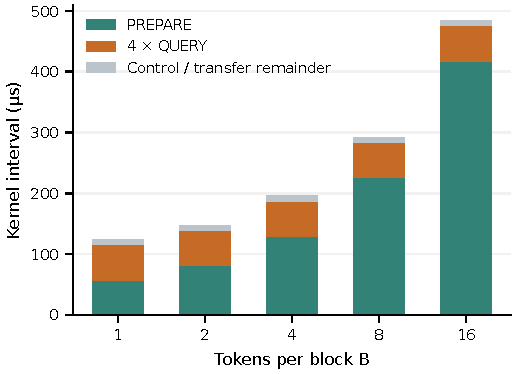
\includegraphics[width=\columnwidth]{latency.pdf}
\caption{Logic Die 模式的时间分解。准备与查询部分来自 RTL 命令计数器，
剩余部分由端到端内核区间相减得到，均按实际 4 ns 门控时钟换算。}
\label{fig:latency}
\end{figure}

软件参考在真实 VORTEX 上执行，但没有使用多 lane、warp 级协作、向量化点积或优化的并行筛选。
硬件与软件还存在频率、存储位置和控制实现差异。因此，表中的时间比较用于检查
当前系统的可执行性与开销组成，不形成对优化 VORTEX、商用 GPU 或端到端 LLM 的加速比结论。
实验采用确定性种子，每组运行一次，并非统计总体上的置信区间估计。

\subsection{标准单元综合开销}
DC 在 28 nm HPC+ 标准单元库的 TT、0.9 V、25\,$^\circ$C 条件下综合完整默认门控顶层。
总映射单元面积为 \AreaMM{} mm$^2$，叶单元数为 \LeafCells{}，无未映射单元。
图~\ref{fig:area} 根据层次面积报告分组，四个权重 bank 及其选择逻辑占
\BankAreaPct{}\%。这个比例反映寄存器实现 8 KiB 多 bank 存储的成本，
不能作为 SRAM 宏实现的面积预测。

在 4 ns 约束下，最差建立裕量为 \SetupSlackPs{} ps，最差保持裕量为
\HoldSlackPs{} ps。保持时间尚未闭合，建立裕量也应结合综合阶段的线负载与理想时钟假设理解。
本文报告映射成功及实际裕量，不宣称布局布线后的 250 MHz 时序闭合。
功耗报告没有工作负载活动标注，故不用于能效比较。

\begin{figure}[t]
\centering
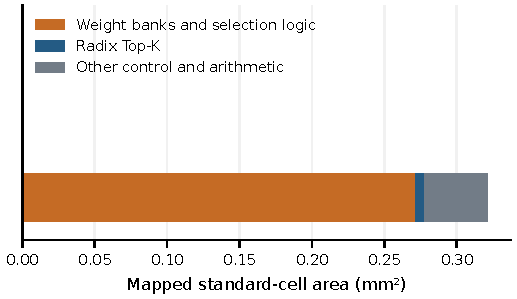
\includegraphics[width=\columnwidth]{area.pdf}
\caption{标准单元层次面积。权重 bank 包含寄存器和读写选择逻辑；
面积不含物理 SRAM 宏、堆叠 DRAM、封装及布局布线后的互连。}
\label{fig:area}
\end{figure}

\section{适用范围与后续工作}
当前结果支持三个有限结论：门控能够在 Logic Die RTL 上完成；真实处理器能通过在线链路
正确提交任务并接收结果；驻留 Kmean 能减少处理器接口上的 K 搬运。
尚不能据此判断完整模型的精度、吞吐率或能效。实验的数据规模、单 lane 软件基线、
串行 AXI 主机和单在途 DMA 都限制了性能结论的外推。

后续物理实现首先需要绑定带端口、时序和功耗模型的 SRAM 或 SRAM-CIM 宏，
比较寄存器基线与宏实现，并完成保持修复、时钟树和布线后的时序检查。
系统层面需增加并发访存、测试主机与门控持续竞争的 QoS，验证显式缓存可见性协议。
算法评估则需要运行真实模型的多 KV 头、长上下文及完整注意力，统计量化门控集合差异。
这些项目未完成前，不使用参考论文或其他平台的数值补齐本文结果。

\section{结论}
本文将 MoBA 的池化、驻留打分和因果 Top-K 落实为堆叠存储 Logic Die 上的数字 RTL，
通过 epoch 限定的复用与独立 DMA 完成路径连接真实 VORTEX 执行。
经数值、事务及负向控制核验，主实验中处理器请求跨度保持在 \HostGateKiB{} KiB，
而 K 数据由本地路径读取。标准单元综合同时暴露了寄存器权重存储成本和未闭合的保持时序。
这为进一步绑定物理存算宏和开展完整模型评估提供了可追溯的工程起点。

\section*{可复现材料与图像来源}
论文的 LaTeX、Python 绘图脚本、精简测量、输入哈希、RTL 和运行入口随功能分支提供。
运行 \texttt{make acceptance} 执行验收；主实验由 \texttt{scripts/experiments.py} 生成；
\texttt{paper/collect\_results.py} 核验并导出图表数据。
图~\ref{fig:concept} 是 AI 辅助概念图，其余架构图和数据图由 Python 生成。
完整波形和日志保留在本地 \texttt{results/}，不将大体积运行日志或专有工艺库纳入 Git。
本文为匿名技术稿，未声明已经投稿或发表。

\bibliographystyle{IEEEtran}
\bibliography{references}
\end{document}
